\section{Xallary: Laborbeispielapp}
Für das bessere Verständis, zeigen von Features und zum einarbeiten in Xamarin haben wir eine App geschrieben, die 
momentan \textbf{unter Android} kompiliert wird, geschrieben.
In dieser App werden die Zugriffe auf die Kamera, auf den Lokalen- und Externenspeicher
gezeigt und wie ein Custom Element geschrieben wird, welches eine feste Android
Implementation ist, da hierbei auf Hardware- und API-Komponenten zugegriffen werden,
die Android spezifisch sind.
\subsection{Aufbau}
Eine Xamarin Applikation hat \textbf{immer} eine feste Grundstruktur, die aus drei Grundprojekten besteht.
Es können natürlich auch weitere Projekte hinzugefügt werden, aber es müssen immer folgende Projekte
vorhanden sein:
\begin{itemize}
    \item Klassenbibliothek
    \item Android, falls nur IOS dann wird das nicht benötigt
    \item IOS, falls nur Android wird dieses nicht benötigt
    \item UWP, dieses Projekt wird benötigt, wenn für Windowsgeräte entwickelt wird. Wie auch bei IOS und Android kann es, falls nicht benötigt, entfertn/deaktiviert werden.
\end{itemize}
(Figure \ref{fig:Ordnerstruktur}) 
\paragraph{Klassenbiliothek} Die Klassebibliothek ist nachdem Projekt benannt. 
Hier also Xallary. Wenn Crossplattformimplementationen 
getätigt werden, was die stärke von Xamarin ist, 
muss das hier geschehen,
da alle Projekte dieses als \textit{Dependency} haben. 
Das einzige, was hier nicht rein sollte und darf, sind Geräte/Betriebssystemabhängige Implementationen, da diese in den anderen Projekten erfolgen müssen.
\paragraph{Android} Sollen Android spezifische Implementationen vorgenommen werden, wie Beispielsweise \textit{Snackbars oder Toasts}, dann 
müssen diese in diesem Projekte implementiert werden. Außerdem muss bei nur androidspezisischen Hardwarekomponenten
diese hier per API Zugriffe implementiert werden. Zumteil sind aber schon Implementation in Xamarin behinhaltet und somit muss dann "nur"
diese in dem Projekt "angemeldet" werden.
\paragraph{IOS} Wie oben bei Android beschrieben, gilt auch hier dass spezfische \textit{OS} Implementation hier vollzogen werden müssen.
\begin{figure}[h]
    \centering
    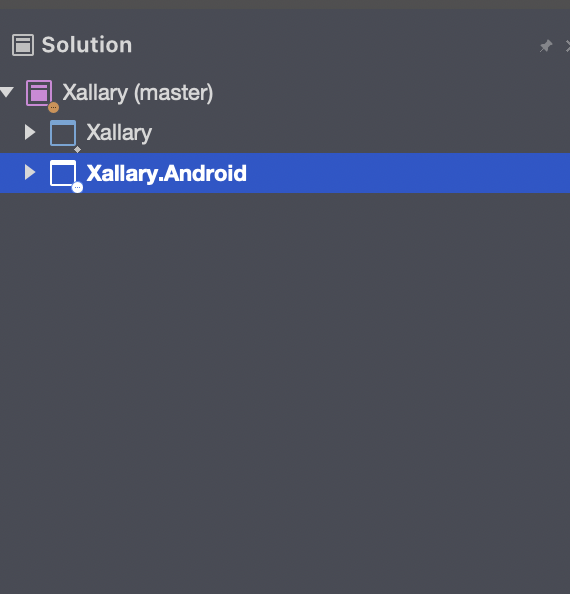
\includegraphics[width=0.9\textwidth]{Bildschirmfoto 2021-05-22 um 23.54.49.png}
    \caption{Orderstruktur von Xallary}
    \label{fig:Ordnerstruktur}
\end{figure}
\subsubsection{Verwendetes Designpattern}
Bei den Designpattern werden verschiedene in diesem Projekt verwendet. 

Zum einen wird das 
\textit{Dependency Injection Pattern} von \textit{Xamarin} verwendet, welches sich um die Verfügbarkeit von Klassen innerhalb
der Unterschiedlichen Projekten kümmert. Das Pattern übernimmt die Verwaltung der Klassen, ob diese bswp. als Singelton implementiert werden soll oder
die Initialisierung und Instanziierung. Dabei werden \textit{Container} erstellt, wo die Klassen
hinein ``exportiert''  werden, die dann wieder durch einen \textit{import} in einer anderen Klasse
importiert werden.(Figure \ref{fig:IoC}, \ref{fig:IoCImport}) 
\begin{figure}[h]
    \centering
    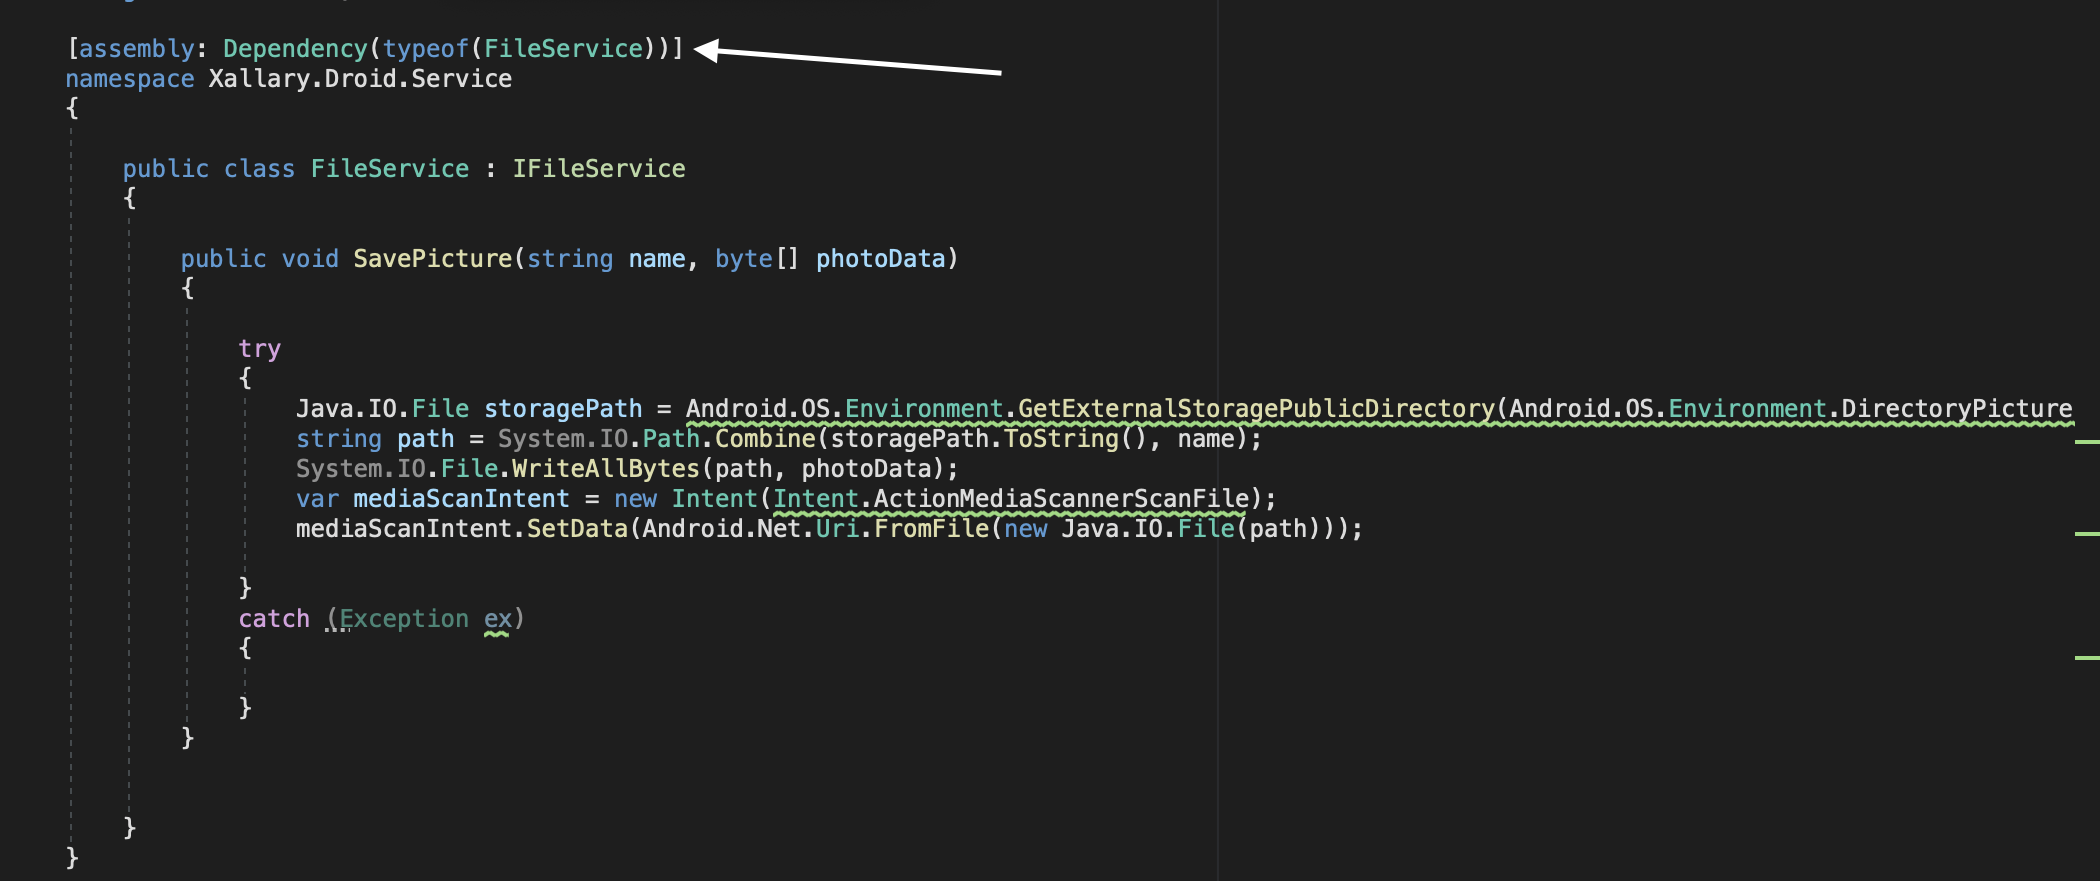
\includegraphics[width=0.9\textwidth]{Bildschirmfoto 2021-05-23 um 00.49.41.png}
    \caption{Attribute Tag für das exportieren einer Klasse in den Container}
    \label{fig:IoC}
\end{figure}

\begin{figure}[h]
    \centering
    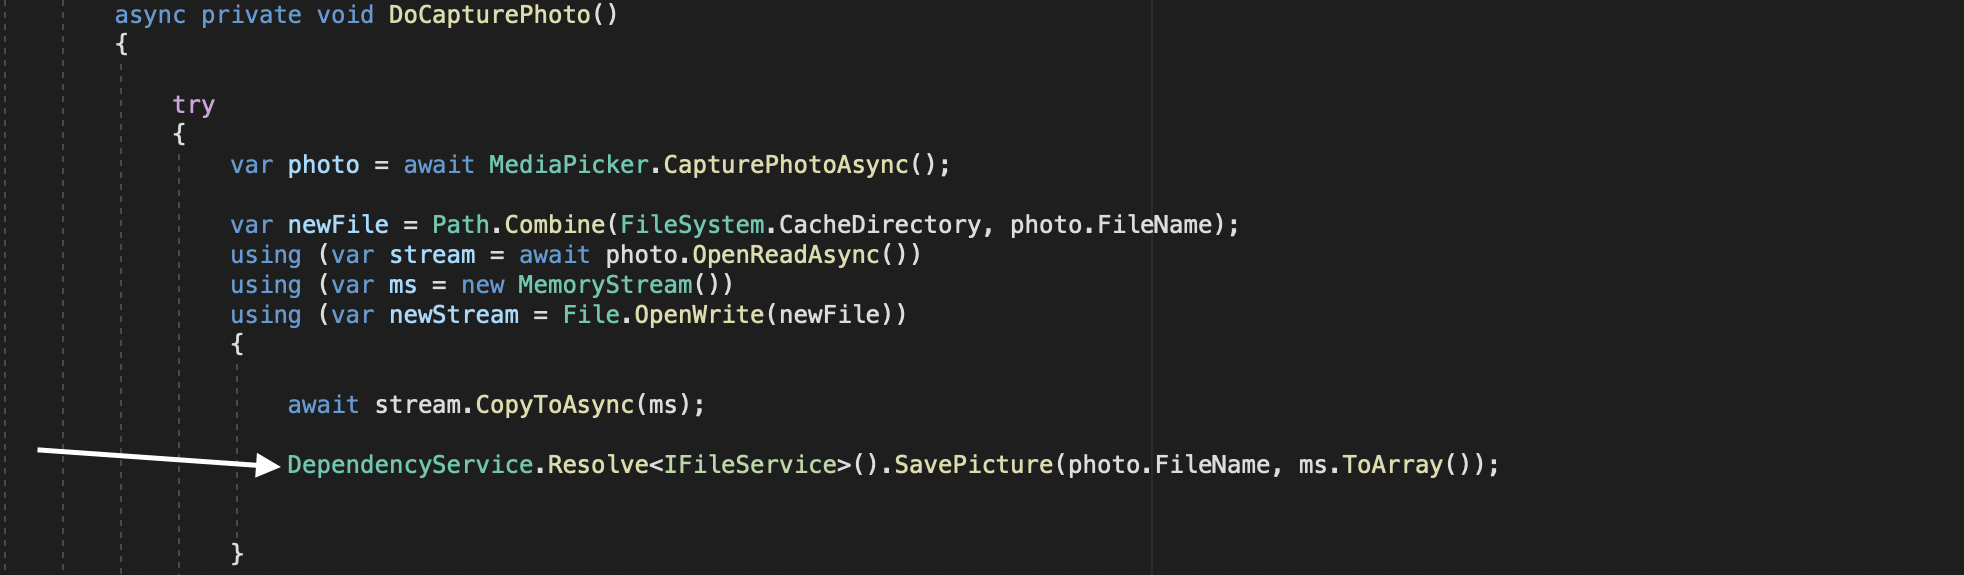
\includegraphics[width=0.9\textwidth]{Bildschirmfoto 2021-05-23 um 01.01.50.png}
    \caption{Verwendung und import der exportierenden Klasse durch ein \textit{Get} }
    \label{fig:IoCImport}
\end{figure}


Als weiteres Pattern wird das \textit{MVVM-Pattern} (Figure \ref{fig:MVVMPattern}), also Model-ViewModel-View, verwendet.
Dieses Pattern ist ein sehr gängiges in der Welt von C\# beziehungsweise von WPF,UWP oder generell Frameworks welches \textit{Xaml} als 
\textit{MarkUpLanugage} verwenden.
\begin{figure}[h]
    \centering
    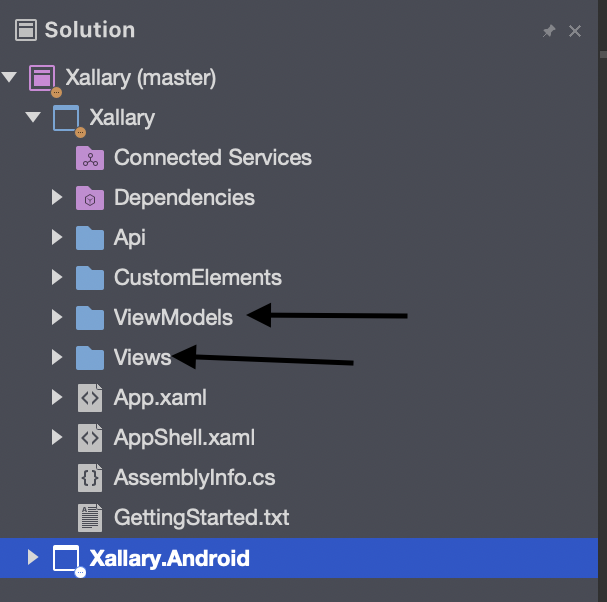
\includegraphics[width=0.9\textwidth]{Bildschirmfoto 2021-05-23 um 00.36.59.png}
    \caption{Orderstruktur des MVVM-Pattern ohne Model}
    \label{fig:MVVMPattern}
\end{figure}

\newpage
Außerdem wird das \textit{Command Pattern} verwendet, welches dafür sorgt, dass die \textit{UI} keinen Code
in der \textit{Code Behind} besitzt, welcher Klickmethoden auslöst.(Figure \ref{fig:CommandXaml})

\begin{figure}[h!]
    \centering
    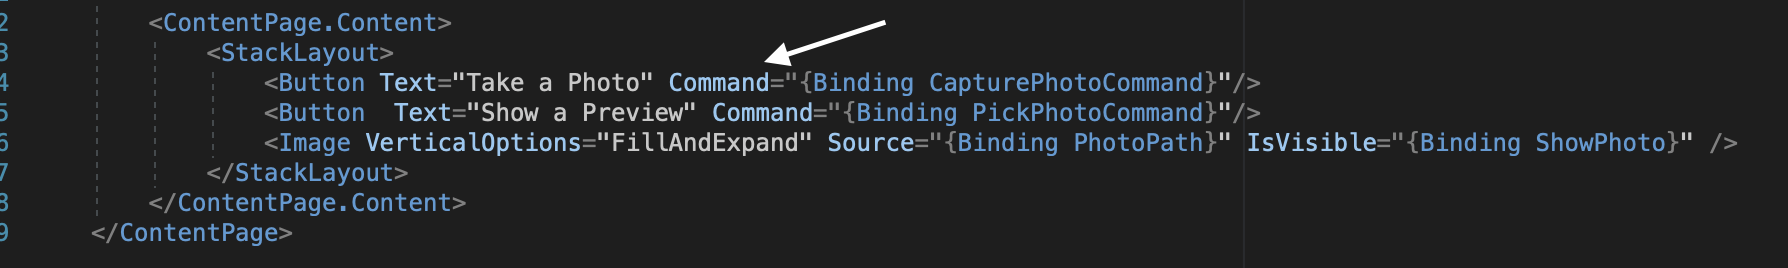
\includegraphics[width=0.9\textwidth]{Bildschirmfoto 2021-05-23 um 01.07.05.png}
    \caption{Verwendung des \textit{Command Property} mit Binding an die Methode im ViewModel}
    \label{fig:CommandXaml}
\end{figure}

\subsection{Permissionverwaltung}
Wie auch in anderen Sprachen muss einer Berechtigung, also ab hier Persmission, eingeholt werden,
damit diverse Ressourcen der Hardware verwendet werden können.
Hier werden folgende Persmission (Figure \ref{fig:Permissions}) benötigt und verwendet:
\begin{itemize}
    \item CAMERA
    \item READ\_EXTERNAL\_STORAGE
    \item WRITE\_EXTERNAL\_STORAGE
\end{itemize}

\paragraph{CAMERA} Diese Persmission wird benötigt, damit die App auf die Kamera zugreifen kann und darf.
Bei Xallary ist es wichtig da das Ziel der Applikation ist, eine funktionierende Foto machene Gallery zu sein.
Ohne diese Persmission ist der App untersagt auf die Kamera zuzugreifen
\paragraph{READ\_EXTERNAL\_STORAGE} Da es sich hierbei um eine Gallerie handelt, muss auch eine Persmission gefordert werden, um auf den Internenspeicher zuzugreifen, um dort
die persitierten Bilder zu laden und dann in der App anzuzeigen.
\paragraph{WRITE\_EXTERNAL\_STORAGE} Wenn Bilder mit der Kamera aufgenommen werden, sollten diese am besten
auch auf dem Gerät oder einem Speichermedium gespeichert werden. Hierbei muss eine Persmission eingeholt werden, die das 
schreiben auf den Speicher des Gerätes erlaubt, da ansonsten keine Bilder wirklich gespeichert werden können und dann nur im \textit{cache}des Gerätes
zwischen gelagert werden.
\begin{figure}[h]
    \centering
    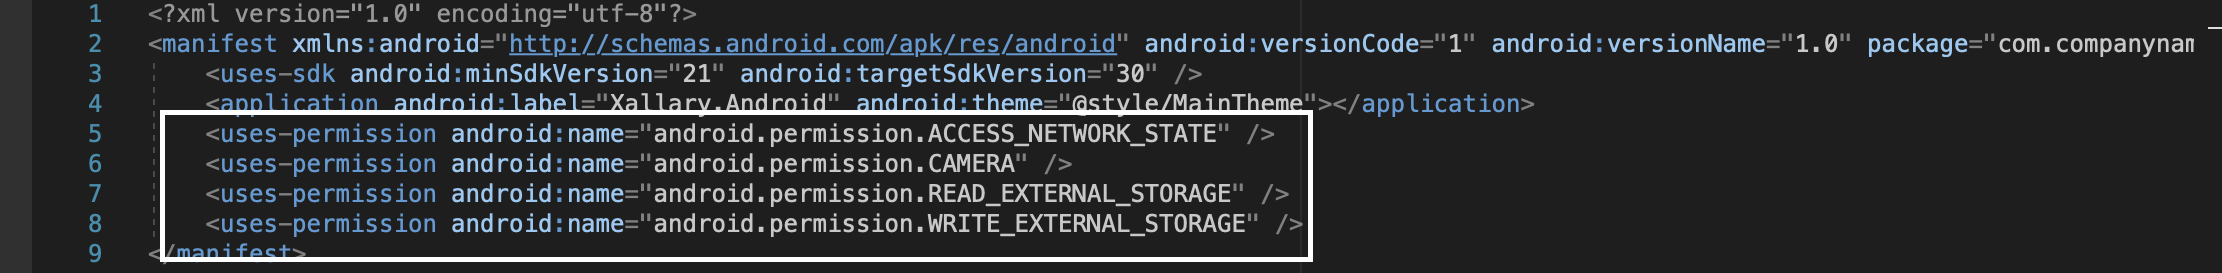
\includegraphics[width=0.9\textwidth]{Bildschirmfoto 2021-05-23 um 01.22.18.png}
    \caption{Gesetzte Permissions in der AndroidManifast.xml}
    \label{fig:Permissions}
\end{figure}
\subsubsection{Benutzer Erfragung für die Permissions}
Damit der Nutzer einer App weiß, welche Freigaben er tätigen muss, wird in der Appentwicklung der Nutzer gefragt,
ob dieser einverstanden ist, dass eine App auf beispielsweise die Kamera zugreifen darf. Verneint dieser diese Anfrage
wird nicht auf die Kamera zugegriffen bis die Persmission von Benutzer erteilt wurde.
Bei \textit{Android} und auch in \textit{Xamarin} muss das Erfragen in der \textit{MainActivity} geschehen. (Figure \ref{fig:MainActivity})

\begin{figure}[h]
    \centering
    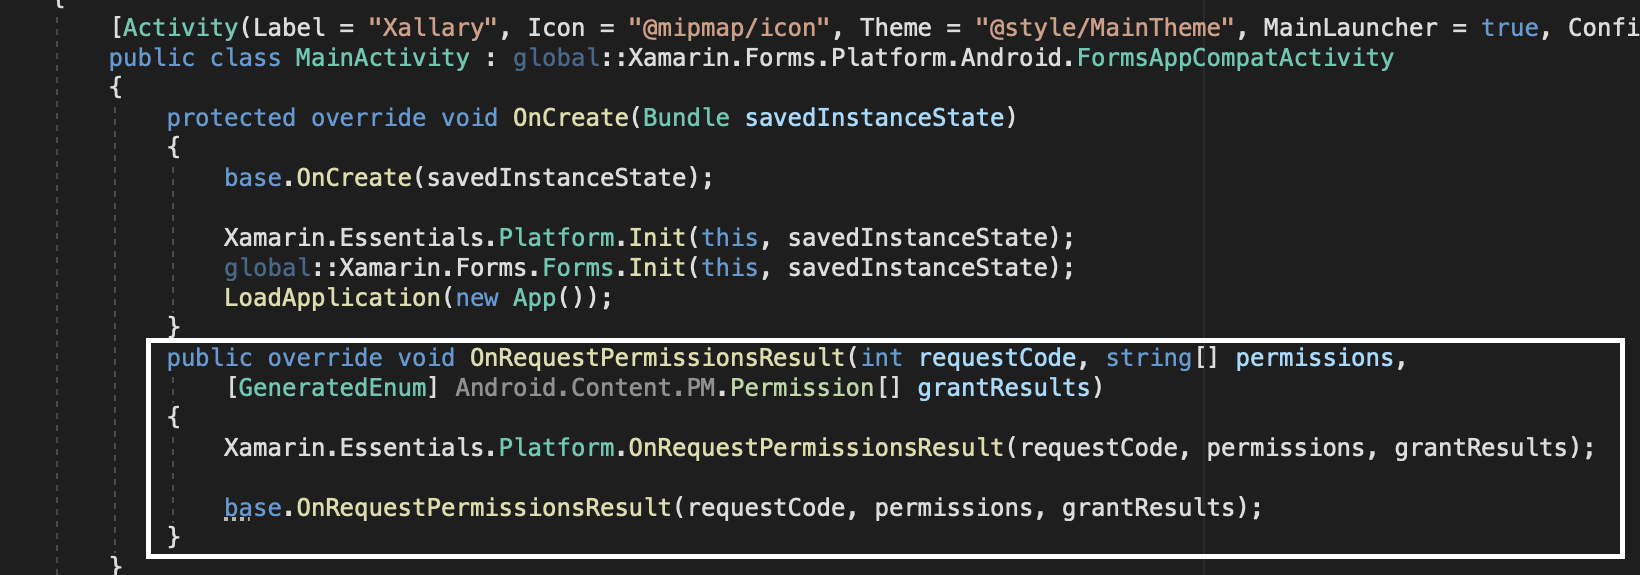
\includegraphics[width=0.9\textwidth]{Bildschirmfoto 2021-05-23 um 02.06.51.png}
    \caption{RequestPermissionMethod in der MainActivity}
    \label{fig:MainActivity}
\end{figure}
\subsection{Customelemente}
Ein \textit{Customelemente} ist wie der Name es sagt, ein individuelles erstelltes Element, welches aus verschiedenen Elementen, wie Button, Grids, Sliders etc.. bestehen kann.
Für eine App ist es wichtig, dass solche Elemente erstellt werden können, da unterschiedliche Anforderungen nicht immer mit den bereits Bereitgesellten Elementen realisiert werden kann.
Außerdem können \textit{Custom Elemente} wiederverwendet werden, was einen \textit{Boiler-Code} im UI-Code erstparrt.
Auch brauchen Entwickler nicht 100x mal die selbe Lösung via \textit{Copy and Paste} einfügen und die Wartbarkeit ist hiermit auch eher gewährleiste, als an 100 Stellen den Code zu modifizieren.

\textit{Customelemente} sind nicht nur ein spezielles Element in \textit{Xamarin} sondern finden auch ihre Verwendung in anderen Sprachen oder 
Frameworks von C\# , wie \textit{WPF} oder \textit{UWP}. 

\subsubsection{Implementation eines Customelementes}
\paragraph{C\#} In C\# werden die Customelemente in einer ``nomalen'' Klasse geschrieben, diese wiederum von der \textit{View-Klasse} erbt, da die \textit{View} die nötigen \textit{Properties} bestitzt.
Außerdem  kann dort ``leichte'' Logik implementiert werden, die eine View benötigt. Um der selbst erstellen \textit{View} eigene, individuelle \textit{Properties}
zu geben, müssen \textit{Bindable Properties} implementiert werden. Diese brauchen bestimmte Parameter. Mehr dazu ist in der Dokumentation zu finden und
bei der Abbildung \ref{fig:CustomelementCS}.

\begin{figure}[h]
    \centering
    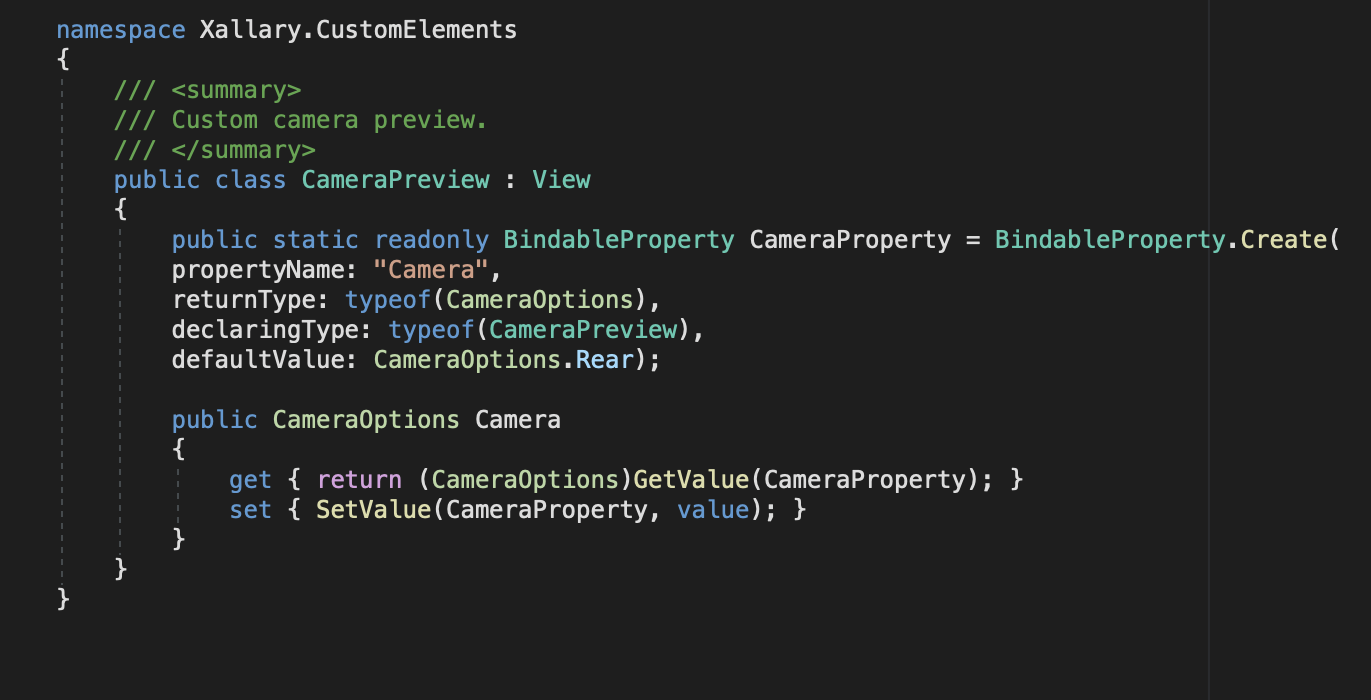
\includegraphics[width=0.9\textwidth]{Bildschirmfoto 2021-05-23 um 18.15.39.png}
    \caption{Customelement Klasse}
    \label{fig:CustomelementCS}
\end{figure} 

Ist das Element korrekt implementiert, kann dieses in jeder \textit{Page/View} verwendet werden, indem das Element
in die \textit{View} importiert wird und dann wie jedes ``normale'' Element verwendet werden. (Figure \ref{fig:UsingCustomElement})

\begin{figure}[h]
    \centering
    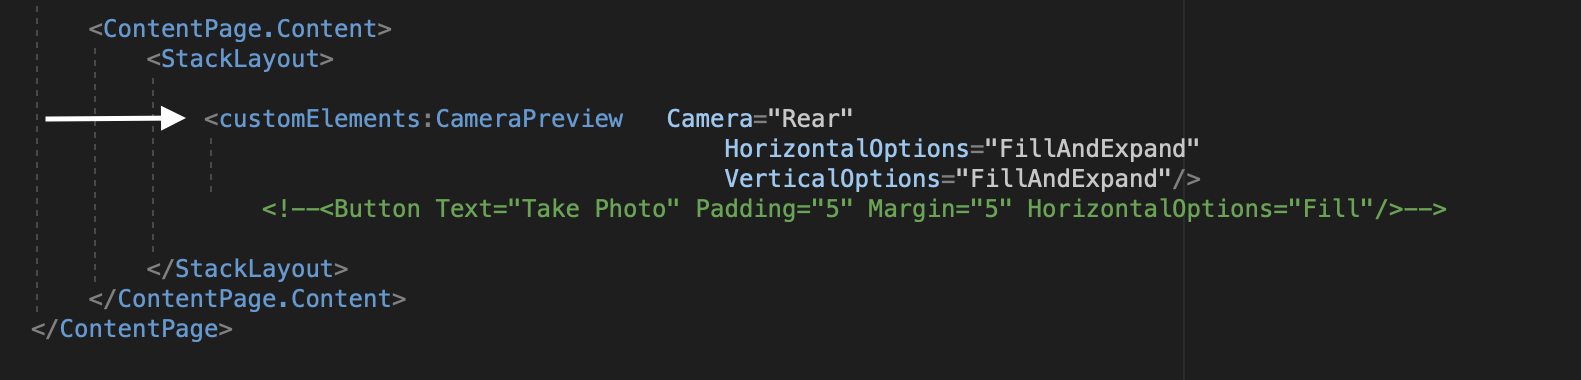
\includegraphics[width=0.9\textwidth]{Bildschirmfoto 2021-05-23 um 18.16.54.png}
    \caption{Verwenden eines Customelementes in einer Page/View}
    \label{fig:UsingCustomElement}
\end{figure}
\paragraph{Android} 
 Die Erstellung eines Customelementes exklusiv für Android ist ein wenig aufwendiger. In unserer App haben wir, das Tutorial von 
\textit{Microsoft} verwendet, welches genau unsere Vorstellungen erfüllt hat. Hier wird ausßerdem noch ein \textit{Custom Renderer} implementiert, der
den C\# Code und den erstellten Andorid Code zusammen ``merged'' und dann die Android Rendermaschine verwendet, um das Element korrekt anzuzeigen.

\subsection{App im Emulator/Smartphone}
Die fertige App sieht wie foglt aus:

\newpage
\subsubsection{Fullscreen Customcameraelemt}
Dieses Element ist das obenbeschriebene \textit{Customelement}.
Zusehen im Bild ist eine Kamera, die von dem Emulator erstellt wurde.
\begin{figure}[h]
    \centering
    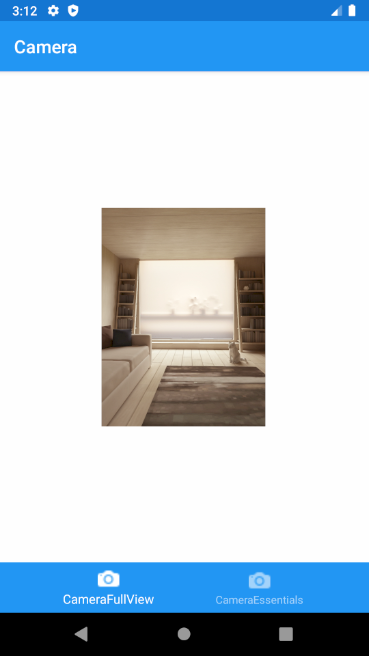
\includegraphics[width=0.5\textwidth]{CustomCameraElement.png}
    \caption{Customelement welches die Kamera des Gerätes verwendet.}
\end{figure}
\subsubsection{Crossplattformimplementationen einer funktionierenden Kamera}
\paragraph{Ansicht ohne ausgewählten oder gemachten Foto}
 Sollte noch kein Foto gemacht worden sein oder ein Foto über das \textit{Filesystem}
 ausgewählt wurde, dann sieht das Element leer aus. Beide Buttons sind im dazugehörogen \textit{Viewmodel} implementiert.
 Die Funktion wurde aus dem Beispiel von Xamarin entnommen und für unsere zwecke angepasst.
\begin{figure}[h]
    \centering
    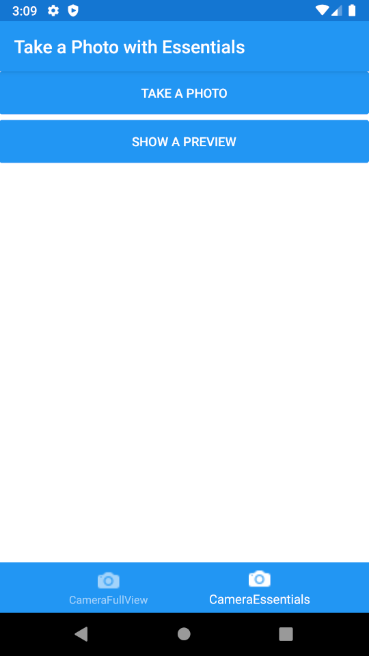
\includegraphics[width=0.4\textwidth]{CleanEssentialsPage.png}
    \caption{Seite mit zwei Buttons, und einem Imageview elementes, welches noch nicht sichtbar ist}
\end{figure}
\newpage
\paragraph{Ansicht mit einem ausgewählten oder gemachten Foto}
 Sollte ein Bild mit der Kamerafunktion gemacht worden oder mit dem Auswahlbutton ausgewählt worden sein,
 wird unter den Buttons dieses Bild erscheinen, da das gewählte \textit{Layout} sich um ein \textit{Stacklayout}
 handelt und dieses ihre Kindelemente übereinander positioniert.
\begin{figure}[h!]
    \centering
    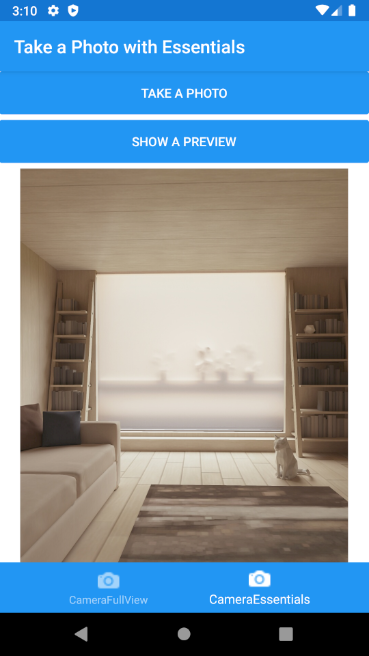
\includegraphics[width=0.6\textwidth]{CameraEssentials.png}
    \caption{Anicht mit Foto}
\end{figure}

\paragraph{Foto schießen}
 Sobald der Button zum Fotomachen gedrückt worden ist, öffnet sich das Betriebssystemkamera-UI
 welches jenach Betriebssystem unterscheidlich aussehen kann. Hier kann dann auf das Fotokamerasymbol
 gedrückt werden und das Foto wird aufgenommen (Figure \ref{fig:TakeFoto}). 
 Nachdem dies gemacht wurde, kommt ein weiterer Dialog, wo der Benutzter entscheiden kann, ob das
 Bild genommen werden soll und somit gespeichert wird oder ob es verworfen werden soll.(Figure \ref{fig:TakeFoto})

 
\begin{figure}[h!]
    \centering
    \begin{subfigure}[b]{0.4\linewidth}
        
\includegraphics[width=\linewidth]{TakePicFromEssentials.png}
      \end{subfigure}
      \begin{subfigure}[b]{0.4\linewidth}
        
\includegraphics[width=\linewidth]{ChoosePic.png}
      \end{subfigure}
    \caption{Foto schießen und auswählen}
    \label{fig:TakeFoto}
\end{figure}

\paragraph{Fotos aus dem \textit{Filesystem} auswählen}
 Um die bereits gemachten Fotos anzuzeigen musst dann auf den anderen Button gedrückt werden.
 Dieser öffnert daraufhin das Filesystem des Betriebssystemes. Dort sind dann die Fotos zusehen, die mit dieser App gemacht wurden.
 Es ist auch möglich Bilder aus der Gallery hier anzuzeigen. (Figure \ref{fig:TakePicFromPicker})

 \begin{figure}[h!]
    \centering
    \begin{subfigure}[b]{0.4\linewidth}
        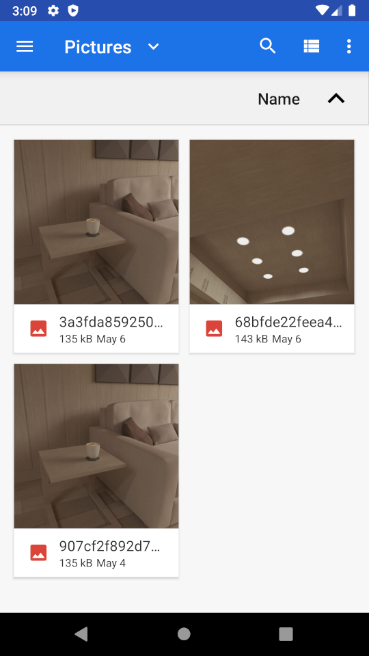
\includegraphics[width=\linewidth]{ChoosePickWithPicPicker.png}
      \end{subfigure}
      \begin{subfigure}[b]{0.4\linewidth}
        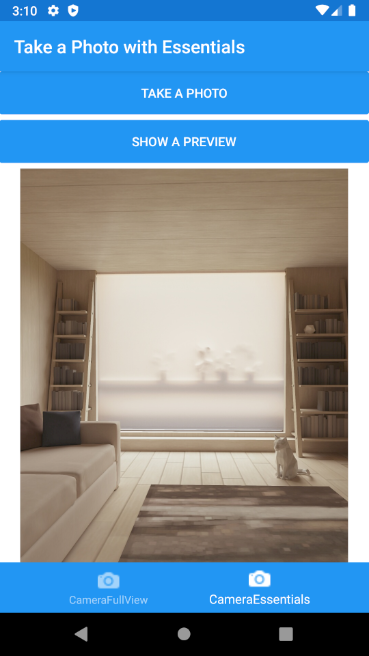
\includegraphics[width=\linewidth]{CameraEssentials.png}
      \end{subfigure}
    \caption{Auswählen und anzeigen eines Fotos}
    \label{fig:TakePicFromPicker}
\end{figure}



